\documentclass[a4paper, 10.5pt, twoside]{jreport}

% include
\usepackage{gra_yasuda}
\usepackage{lscape}
\usepackage{graphicx}
\usepackage{here}
\usepackage{color}
\usepackage{amsmath}
\usepackage{subfig}
\usepackage{tascmac}
\usepackage{url}
\usepackage{ascmac}
\usepackage{booktabs}
\usepackage{otf}
\usepackage{comment}



%タイトル
\title{心理的効果を用いた人間とエージェントの繰り返し交渉戦略}
\etitle{Repetitive negotiation strategy of human and agent \\ using psychological effect}

%名前
\author{松下 昌悟}
\eauthor{Shogo MATSUSHITA}

%入学年度
\enteryear{2017}
%卒業年度
\graduateyear{2018}

%学籍番号
\studentnumber{17268508}

%提出日
\date{平成30年1月31日}

\begin{document}

%ここで行ピッチを指定
%フォントを変えるとサイズがリセットされてしまうので注意
\setlength{\baselineskip}{8truemm}


%ここから内容

% Chapter 2
\chapter{関連研究}\label{cha:2}

\section{自動交渉エージェント競技会(ANAC)}

\subsection{ANAC}
自動交渉エージェント競技会(Automated Negotiation Agent Competition)\cite{iago}

\subsection{IAGO}
IAGO(Interactive Arbitration Guide Online)はANACのHuman-agent Negotiationリーグで使用される自動交渉のプラットフォームである.
IAGOのインタフェースを図\ref{fig:iago}に示す.IAGOでは,人間と交渉を行うエージェントおよび交渉のドメインを作成することが可能である.IAGOの特徴として以下の3点が挙げられる\cite{pinocchio}.

\begin{enumerate}
  \item WEB上で動作する
  \item APIが公開されている
  \item 人間同士の交渉で用いられるチャネルが利用可能
\end{enumerate}

第1の特徴により,エージェントと交渉を行うクライアントはWEBブラウザ上で交渉を行うことが可能である.
したがって,クライアントはソフトウェアのインストールなどを行うことなく交渉を開始することができる.
第2の特徴により,競技会や研究のためのエージェントおよび交渉ドメインの設計を容易に行うことが可能となる.
第3の特徴により,エージェントおよびクライアントは感情の表出,メッセージの送信,選好の公開および誘発などを交渉中に行うことが可能となる.
これにより,人間同士の交渉で用いられるチャネルによる交渉結果への影響を研究することおよび
これらのチャネルを利用した交渉を行うエージェントを作成することが容易となる.

\begin{figure}[h]
  \centering
  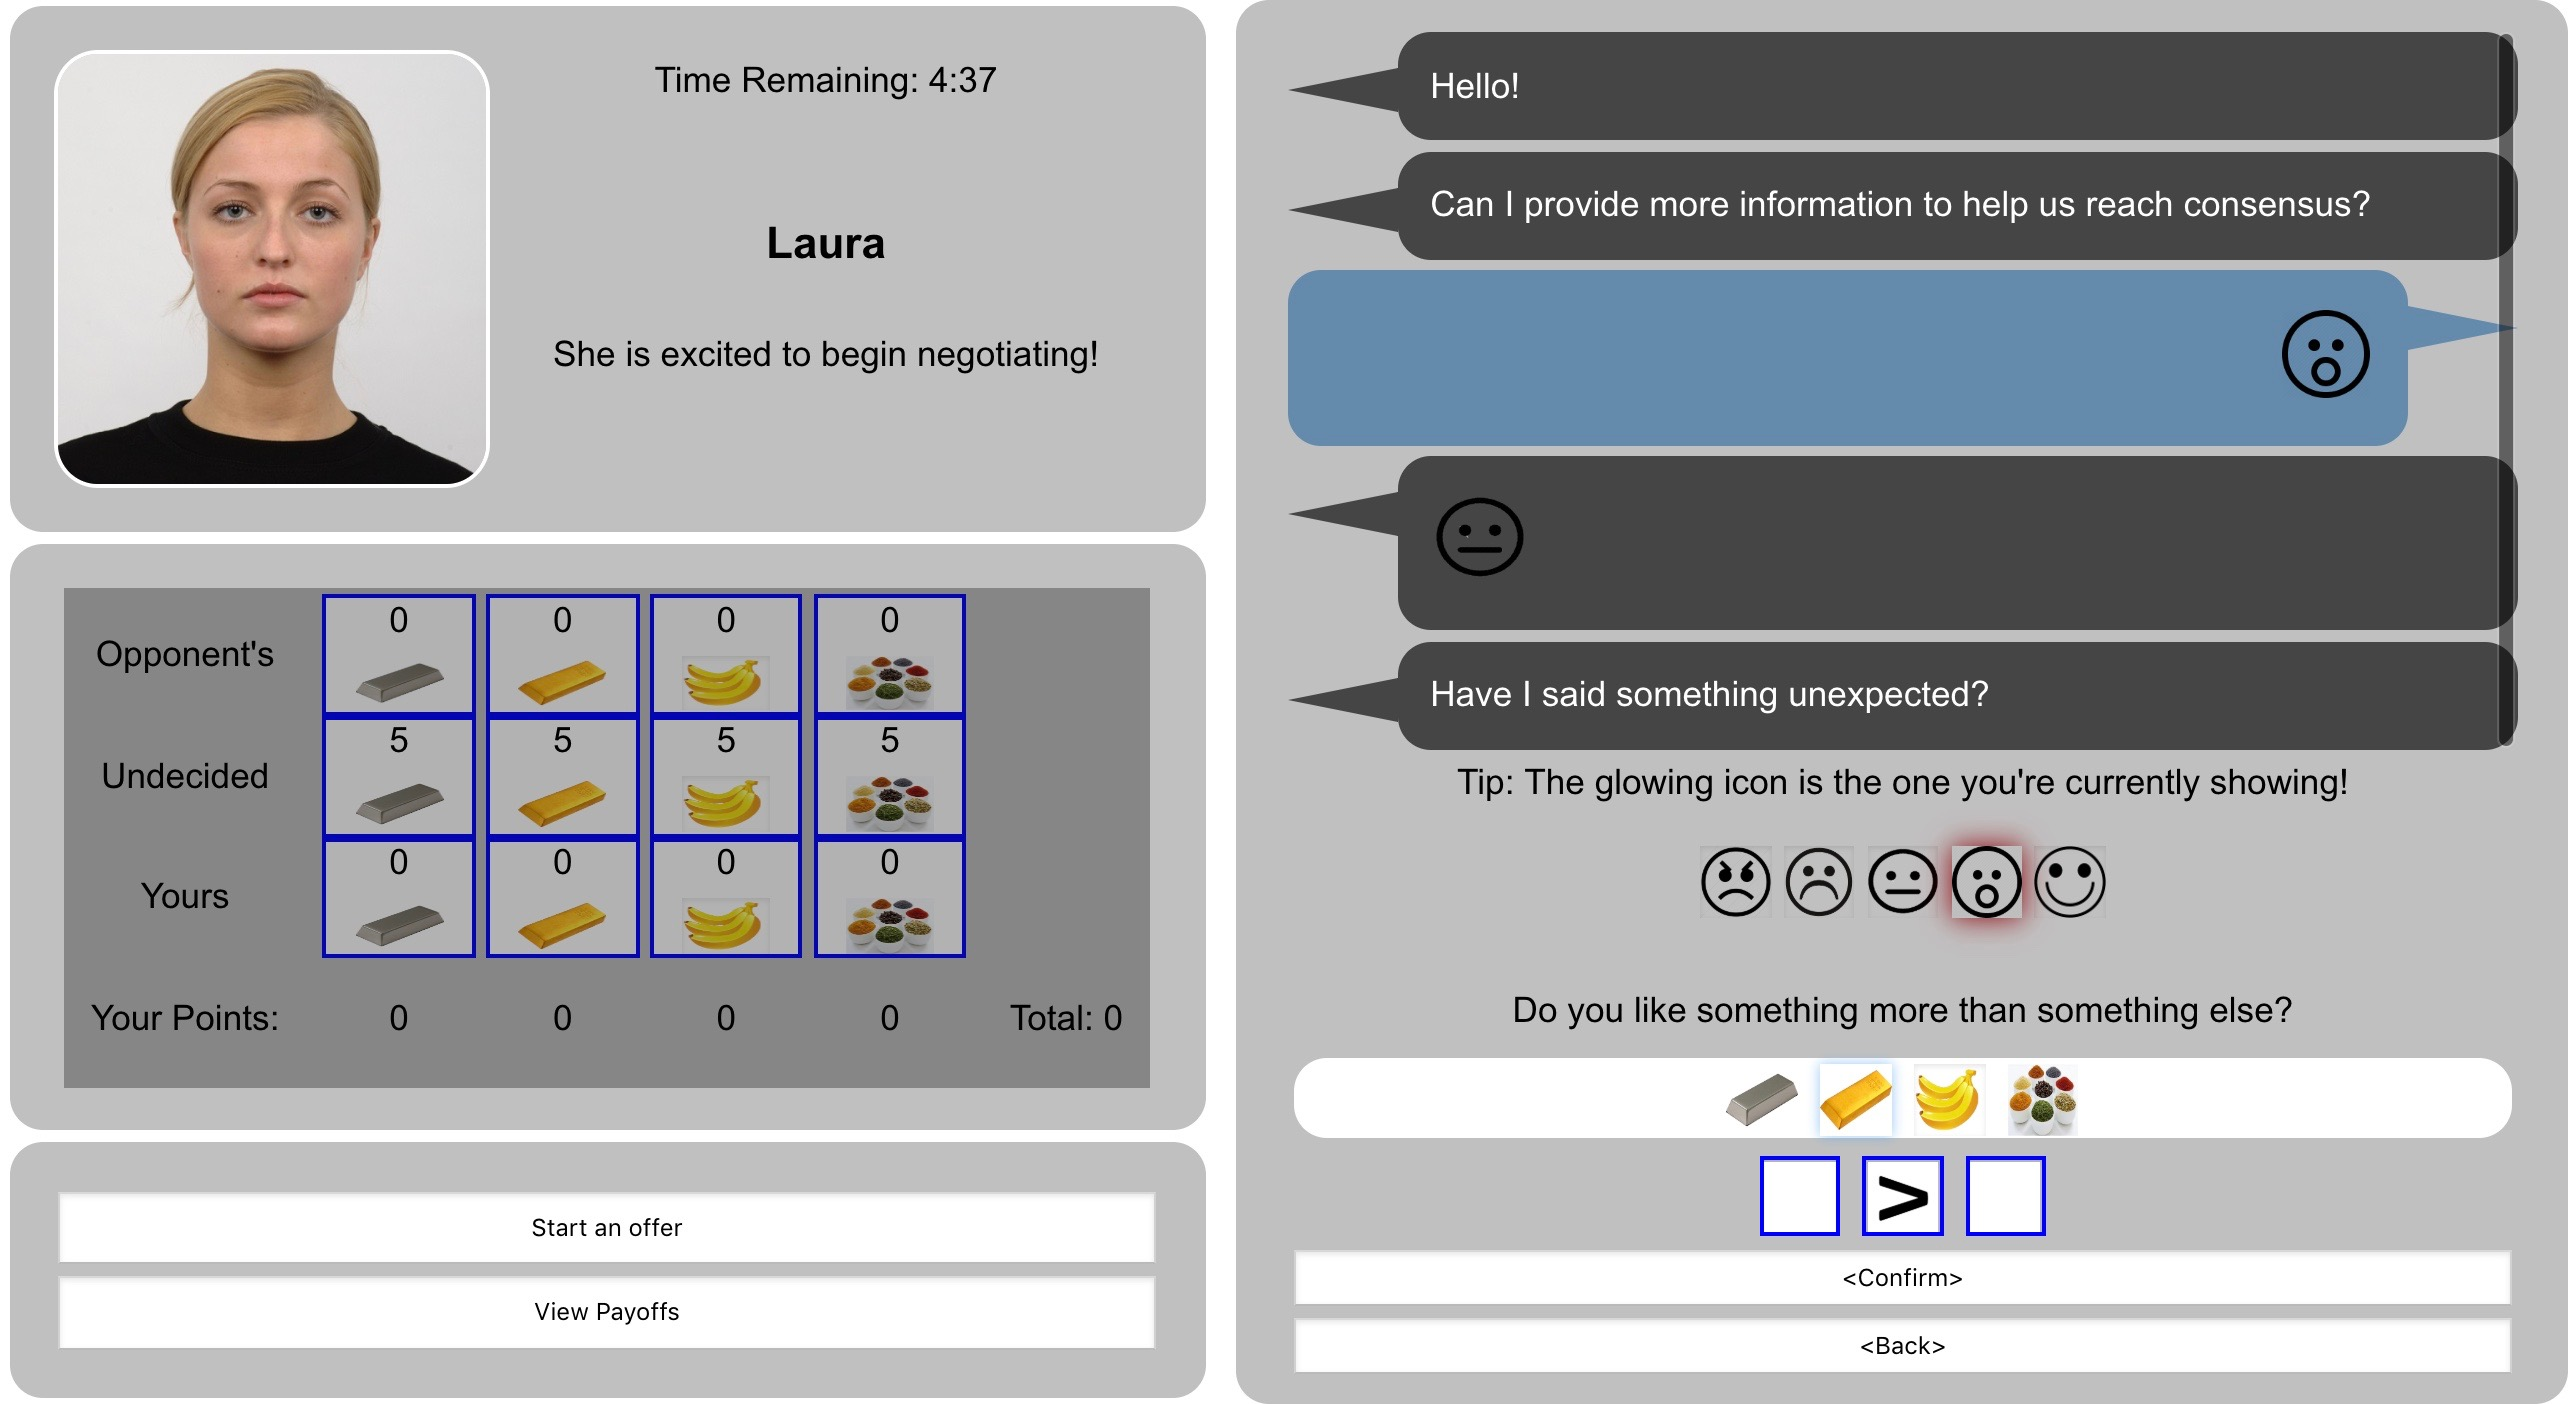
\includegraphics[width=15truecm]{image/IAGO.eps}
  \caption{IAGOのインタフェース}
  \label{fig:iago}
\end{figure}

%内容ここまで

\chapter*{謝辞}
本論文を執筆するにあたり,多数の方々からご指導・ご協力いただきましたことを,心より御礼申し上げます.

指導教員である藤田桂英准教授には,研究の機会を与えていただき,研究の方針に関する助言や発表練習等の
多大なるご指導や助言をいただきましたことを深く感謝いたします.

研究に関する知識のご教示に加えて,本実験の準備を行うにあたってWEBサーバを構築する際にお力添えいただいた松根鷹生様に深く感謝申し上げます.
また,藤田桂英研究室の皆様には研究に必要な知識や意見等をいただいたことを心より感謝いたします.

本実験を行うにあたってお忙しい中ご協力いただいた同期の編入生の方々,および安井貴規様がいなければ本論文は完成に至りませんでした.
心より御礼申し上げます.

最後に,様々な面で私を支えていただいた家族に,心より感謝いたします.ありがとうございました.

\bibliographystyle{plain}
\bibliography{reference}


\begin{comment}
%付録で発表論文をつけてアピールだ!!

\renewcommand{\bibname}{付録 発表論文一覧}
%\chapter{発表論文一覧}

\begin{thebibliography}{99}
\item S. Kakimoto and K. Fujita. 二者間複数論点交渉問題におけるパレートフロント推定手法の提案. Joint Agent Workshop and Symposium, 2014.
\item S. Kakimoto and K. Fujita. Estimating Pareto Fronts using Interdependency between Issues for Bilateral Multi-issue Closed Nonlinear Negotiations. Applications Knowledge and Service Technology for Life, Environment, and Sustainability workshop(KASTLES),2014.
\item S. Kakimoto and K. Fujita. 二者間非線形交渉問題におけるパレートフロント推定を利用した自動交渉エージェントの設計と評価. 情報処理学会 第177回 知能システム研究会, 2014.

\end{thebibliography}

\end{comment}

\end{document}

